% =====================================================================
%  Chapter 10 — Energy and the Hazard Class
% =====================================================================

\chapter{Energy and the Hazard Class}
\label{ch:energy}

The chain now closes. A size, a density and an impact speed\idx{Impact speed} give an energy;
the energy and the probability give a hazard class. This chapter assembles
the chain, puts a number on what is left over, and states what the leftovers
are worth in the only currency that matters, which is how often objects of
that energy actually arrive.

\section{Assembling the chain}

From \eqref{eq:energy},
\begin{equation}
E = \frac{1}{2}\,\rho\,\frac{\pi}{6}\,D^{3}\,v^{2},
\label{eq:energy2}
\end{equation}
with \(D\) the effective diameter in metres, \(\rho\) the bulk density in
kilogrammes per cubic metre and \(v\) the impact speed\idx{Impact speed} in metres per second,
the energy in joules. Divide by \(4.184\times 10^{15}\) joules per megaton
and the number is in megatons.

The impact speed\idx{Impact speed} is the one term that is not in doubt. It is the vector sum
of the object's heliocentric orbital velocity and the Earth's, and for a
near-Earth object on an eccentric orbit that meet the Earth's velocity
vector at some angle, the collision speed at the Earth is typically 14 to 17
kilometres per second. For the 2024~YR4 lunar impact, the published value is
14.1 kilometres per second. At that speed the energy per unit mass is
\(v^{2}/2 = 9.95\times 10^{7}\) joules per kilogramme, so the energy of an
impact is numerically close to the mass in kilograms multiplied by a hundred
million --- which is the reason the energy is so sensitive to the mass.

\begin{table}[!htbp]
\centering
\small
\caption{Energy against size for the impact speeds of interest, at a bulk
density of 2,500 kilogrammes per cubic metre.}
\label{tab:energy-table}
\begin{tabularx}{\textwidth}{@{}P{0.88in}P{0.91in}P{0.91in}Y@{}}
\toprule
\rowcolor{panel}
\textbf{Diameter} & \textbf{At 14.1 km/s} & \textbf{At 17 km/s} &
\textbf{Characteristic} \\
\midrule
30 m & 0.11 Mt & 0.17 Mt & city scale \\
\rowcolor{panel}
60 m & 0.90 Mt & 1.39 Mt & regional, the 2024 YR4 class \\
140 m & 6.9 Mt & 10.7 Mt & the catalogue's threshold class \\
\rowcolor{panel}
325 m & 195 Mt & 302 Mt & Apophis \\
1 km & 5,790 Mt & 8,960 Mt & global \\
\bottomrule
\end{tabularx}
\end{table}

The 140-metre row is the reason the catalogue's threshold class is the one
the book uses. At a bulk density of 2,500 and 14 kilometres per second, a
140-metre object delivers nearly seven megatons --- regional devastation.
Halve the density to the rubble-pile value and the same object delivers three
megatons; double it to a coherent body and it delivers fifteen. The
characterisation of the object moves it across the boundary between the
class of events that empty a hospital and the class that level a city.

\section{The hazard class, and what the scale actually computes}

The Torino scale is a communication instrument with two axes, and Chapter 2
took it apart. It is worth restating here what it does with the energy this
chapter computes, because the scale's structure is the reason the energy
uncertainty matters.

The scale's levels 2 and 3 concern objects whose impact would cause
localised destruction and whose probability of impact is below and above one
per cent respectively. Levels 4 through 8 describe collisions that are
certain or near-certain, with the effect running from regional to global.
Level 9 is a certain collision capable of global climatic catastrophe, and
level 10 is reserved for the extinction case.

The level boundaries are defined in terms of the pair \((p, E)\), and the
Level 1 boundary --- the threshold at which an object begins to merit formal
attention --- is the line
\begin{equation}
p \geq \frac{4.64\times 10^{-3}}{E},
\label{eq:level1b}
\end{equation}
as derived in Chapter 2 from the scale's defining inequality. The
consequence is immediate and unforgiving: the probability at which an object
becomes a notification event is set by the energy, and the energy is the
quantity the catalogue does not contain.

\begin{figure}[!htbp]
\centering
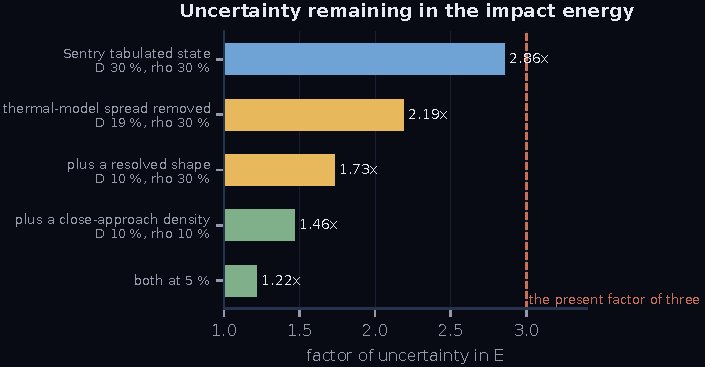
\includegraphics[width=\textwidth]{../figures/fig_energy_ladder.pdf}
\caption{What each link of the energy chain is worth. The present state of
the art leaves a factor of 2.86; removing the thermal-model ambiguity
removes about a quarter of it, and the density term accounts for most of the
remainder.}
\label{fig:energy-ladder}
\end{figure}

\figref{fig:energy-ladder} is the managerial summary of Part II. Each bar is
the factor by which the impact energy remains uncertain once the stated
measurements are in hand. The first bar reproduces the field's own published
statement --- a factor of three --- which is a useful check that the
arithmetic is calibrated against something outside this book.

The decomposition matters more than the total. Removing the thermal-model
ambiguity, by measuring the shape directly, takes the factor from 2.86 to
2.19. Adding a density from a close-approach mass takes it to 1.46. The
remaining gap is the difference between a hazard class that is assigned and
one that is known.

\section{How often this happens}

An energy is only meaningful against a rate of arrival. The European Space
Agency's Near-Earth Object Coordination Centre's background-impact model
gives the frequency \(f_b\) of impacts of a given energy as
\begin{equation}
f_b \approx 0.03\,E^{-0.8}
\quad \mathrm{per\ year},
\label{eq:background}
\end{equation}
with \(E\) in megatons. The model is steeply decreasing, which is the point:
the energies that dominate the casualty risk are the ones that arrive least
often, and they are also the ones the catalogue characterises worst.

\begin{table}[!htbp]
\centering
\small
\caption{Background impact frequency against energy, from the ESA Near-Earth
Object Coordination Centre model.}
\label{tab:background}
\begin{tabularx}{\textwidth}{@{}P{1.16in}P{1.40in}Y@{}}
\toprule
\rowcolor{panel}
\textbf{Energy} & \textbf{Frequency} & \textbf{One impact per} \\
\midrule
\(10^{-3}\) Mt & \(2.4\times 10^{-2}\) a year & 42 years \\
\rowcolor{panel}
\(10^{-2}\) Mt & \(5.9\times 10^{-3}\) a year & 170 years \\
\(10^{-1}\) Mt & \(1.5\times 10^{-3}\) a year & 700 years \\
\rowcolor{panel}
1 Mt & \(3.0\times 10^{-4}\) a year & 3,300 years \\
6.5 Mt & \(8.4\times 10^{-5}\) a year & 12,000 years \\
\rowcolor{panel}
\(10^{2}\) Mt & \(2.5\times 10^{-5}\) a year & 40,000 years \\
\(10^{6}\) Mt & \(7.5\times 10^{-7}\) a year & 1.3 million years \\
\bottomrule
\end{tabularx}
\end{table}

Two observations follow. The first is that the events in the 140-metre class
arrive roughly once in twelve thousand years, which is exactly the timescale
over which the astrometric uncertainty at long horizons has to be defended.
The second is that the probability of any particular object being the one
that hits is small --- but the number of objects that could be the one that
hits is large, and the population of uncharacterised objects is 9,966
objects in the hazard class that have no physical account at all.

\section{The chain, closed and annotated}

\begin{table}[!htbp]
\centering
\small
\caption{The accountability chain, with the measurement that closes each
link and what the link is currently worth.}
\label{tab:accountability-chain}
\begin{tabularx}{\textwidth}{@{}P{1.24in}P{1.32in}Y@{}}
\toprule
\rowcolor{panel}
\textbf{Link} & \textbf{Closed by} & \textbf{Status} \\
\midrule
Shape to volume & resolved imaging & available, at a scale nothing is
currently assigned to \\
\rowcolor{panel}
Volume to mass & bulk density & unresolved; a factor of 2.7 \\
Mass to energy & impact speed & well determined \\
\rowcolor{panel}
Energy to hazard class & the scale's definitions & exact, given the energy \\
\bottomrule
\end{tabularx}
\end{table}

\begin{keytakeaways}
\item A 140-metre object delivers several megatons at typical impact
speeds, and the choice between a rubble pile and a coherent body moves it
across the threshold between local and regional damage.
\item The Level 1 notification threshold is proportional to the inverse of
the energy, so the energy uncertainty moves the notification boundary.
\item Removing the thermal-model ambiguity takes the residual energy factor
from 2.86 to 2.19; adding a close-approach density takes it to 1.46.
\item Background impacts at these energies arrive once in twelve thousand
years, which is the same timescale as the astrometric uncertainty the
community must defend.
\end{keytakeaways}
